\documentclass[12pt]{article}

\usepackage{sbc-template}
\usepackage{graphicx,url}
\usepackage[utf8]{inputenc}
\usepackage[brazil]{babel}
%\usepackage[latin1]{inputenc}  
\usepackage{setspace}
     
\sloppy
\title{Pipeline: Uma Técnica de Programação Paralela}
\vspace{0.5cm}
\author{Erick Modesto Campos}
\vspace{0.5cm}

\address{Instituto de Ciência Exatas e Naturais (ICEN) -- Universidade Federal do Pará
  (UFPA)\\
  Laboratório de Visualização, Interação e Sistemas Inteligentes (LabVis - UFPA)\\
  Cep 66075110 -- Belém -- Pará -- Brazil
  \email{erick.c.modesto@gmail.com / erickcampos@ufpa.br}
}


\begin{document} 

\onehalfspace
\maketitle

\begin{abstract}
   With the evolution of microprocessors, the execution of sequential tasks has
   become increasingly unfeasible to be applied in scenarios where the issue of
   performance must be considered. Therefore, parallel programming techniques
   are essential to extract maximum performance in sequential task tasks.
   Therefore, parallel programming techniques are essential to extract maximum
   performance in serial tasks. In this sense, the so-called pipeline technique
   may be a good alternative for improving performance in applications.

\end{abstract}
     
\begin{resumo}
  Com a evolução dos microprocessadores, a execução de tarefas sequenciais foi
  se tornanando cada vez mais inviável de ser aplicado em cenários onde a
  questão do desempenho deve ser considerado. Por isso, técnicas de programação
  paralela são imprescindíveis para extrair o máximo de desempenho em tarefas
  de tarefas sequenciais. Nesse sentido, a técnica denominada de pipeline pode
  ser uma boa alternativa para a melhora de desenpenho em aplicações.
\end{resumo}

\begin{section}{Introdução}
O processamento de imagens é um método que executa uma série de operações
matemáticas em uma imagem. O intuito é obter um aprimoramento ou extrair algumas
informações úteis a cerca da imagem a ser processada. Esse método nada mais é do
que um processamento digital de sinais onde a entrada é uma imagem e a saída
pode ser uma imagem ou características (\textit{features}) associadas com a
determinada imagem processada~\cite{Tartu19}.

A área de processamento de imagens existem diversos algoritmos que são
utilizados para diversos propósitos. O reconhocimento de objetos é um bom
exemplo de aplicação das técnicas de processamento. No entanto, assim como
outros algoritmos, é necessário realizar várias aplicações chamadas de
pré-processamento. E geralmente os sistemas que implementam o reconhecimento de
objetos em uma imagem, utilizam conversão da imagem original para a escala de
cinza como primeira etapa de pré-processamento.

\end{section}
\begin{section}{Pipelining}
Pipeline é uma técnica bem antiga e bastante conhecida por ser empregada na
linha de produção industrial. A ideia por trás dessa técnica é bastante simples.
Um processo passa por vários estágios da linha de montagem, subdividindo em
tarefas menores, e essa linha de montagem é continuamente alimentada de novos
processos. Em cada estágio uma parte de um processo é finalizado e passado para
o próximo estágio. Quando é chegado no ultimo estágio, cada subprocesso
finalizado é reunido e então finalmente finalizado
completamente~\cite{Bhujade95}. Um bom exemplo da aplicação dessa técnica é na
industria automobilística onde são construídos diversos carros simultaneamente.
A Figura~\ref{fig:carro} mostra a ilustração da aplicação do pipeline na linha
de montagem de um carro.

\begin{figure}[!h]
	\centering
	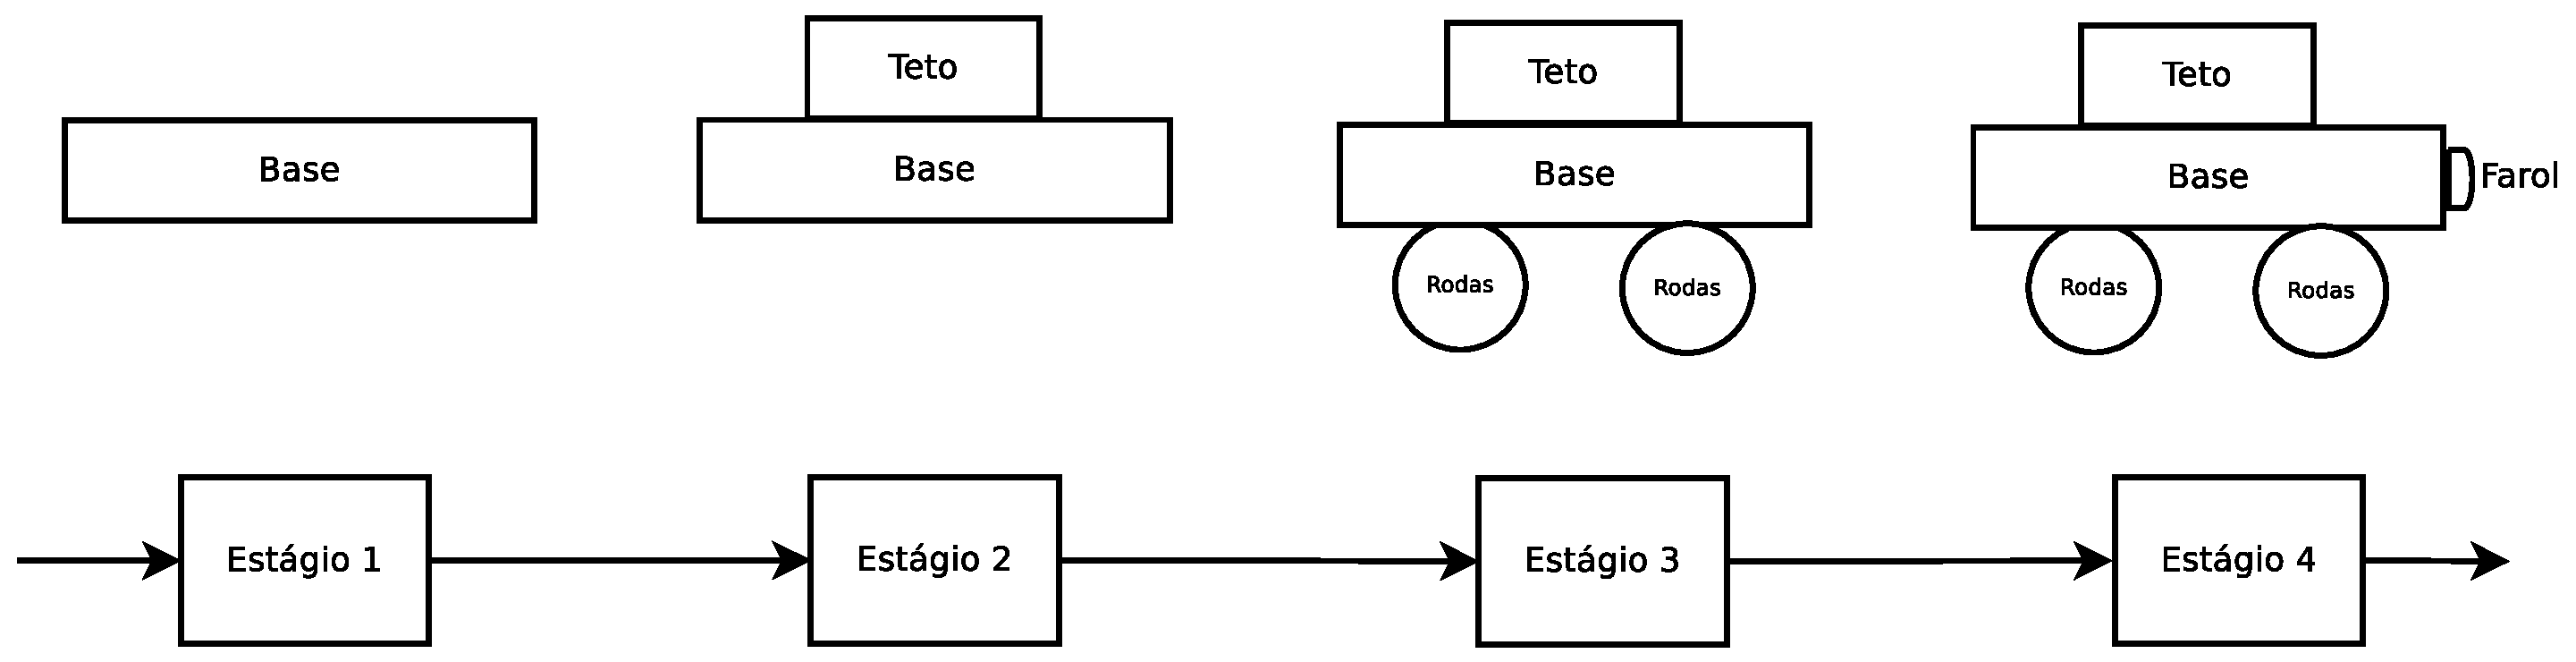
\includegraphics[width=0.95\linewidth]{figs/carro}
	\caption{Processo de uma linha de montagem da industria automobilística.}
	\label{fig:carro}
\end{figure}

Na computação essa técnica foi também incorporada para o desenvolvimento de
programas. Com a grande variedade de processadores multicore, houve a
necessidade de aproveitar ao máximo o poder de processamento de cada núcleo do
processador. A execução de tarefas sequenciais não é a melhor forma de obter
alto desempenho de processamento. Nesse sentido, o pipelining se torna uma
técnica alternativa para aumentar o desempenho de tarefas sequenciais de
\textit{software}.

Ao utilizar a técnica de pipelining, um processo que normalmente seria
executado de forma sequencial é dividido em estágios distintos que podem ser
executados em um modelo de linha de montagem semelhante ao exemplo mostrado
anteriormente, onde dada núcleo do processador fica encarregado de executar uma
subtarefa. 

Dessa forma, o pipelining melhora o desempenho, pois a subdivisão de uma tarefa
em tarefas menores executadas cada uma por um certo processador é mais rápido
para ser finalizada que se cada uma das subtarefas fossem executadas apenas por
um único processador.

É importante ressaltar que para haver uma melhora significativa no desempenho, é
sempre recomendável manter o balanceamento das subtarefas. A
Figura~\ref{fig:bal} mostra a questão do balanceamento.

\begin{figure}[!h]
	\centering
	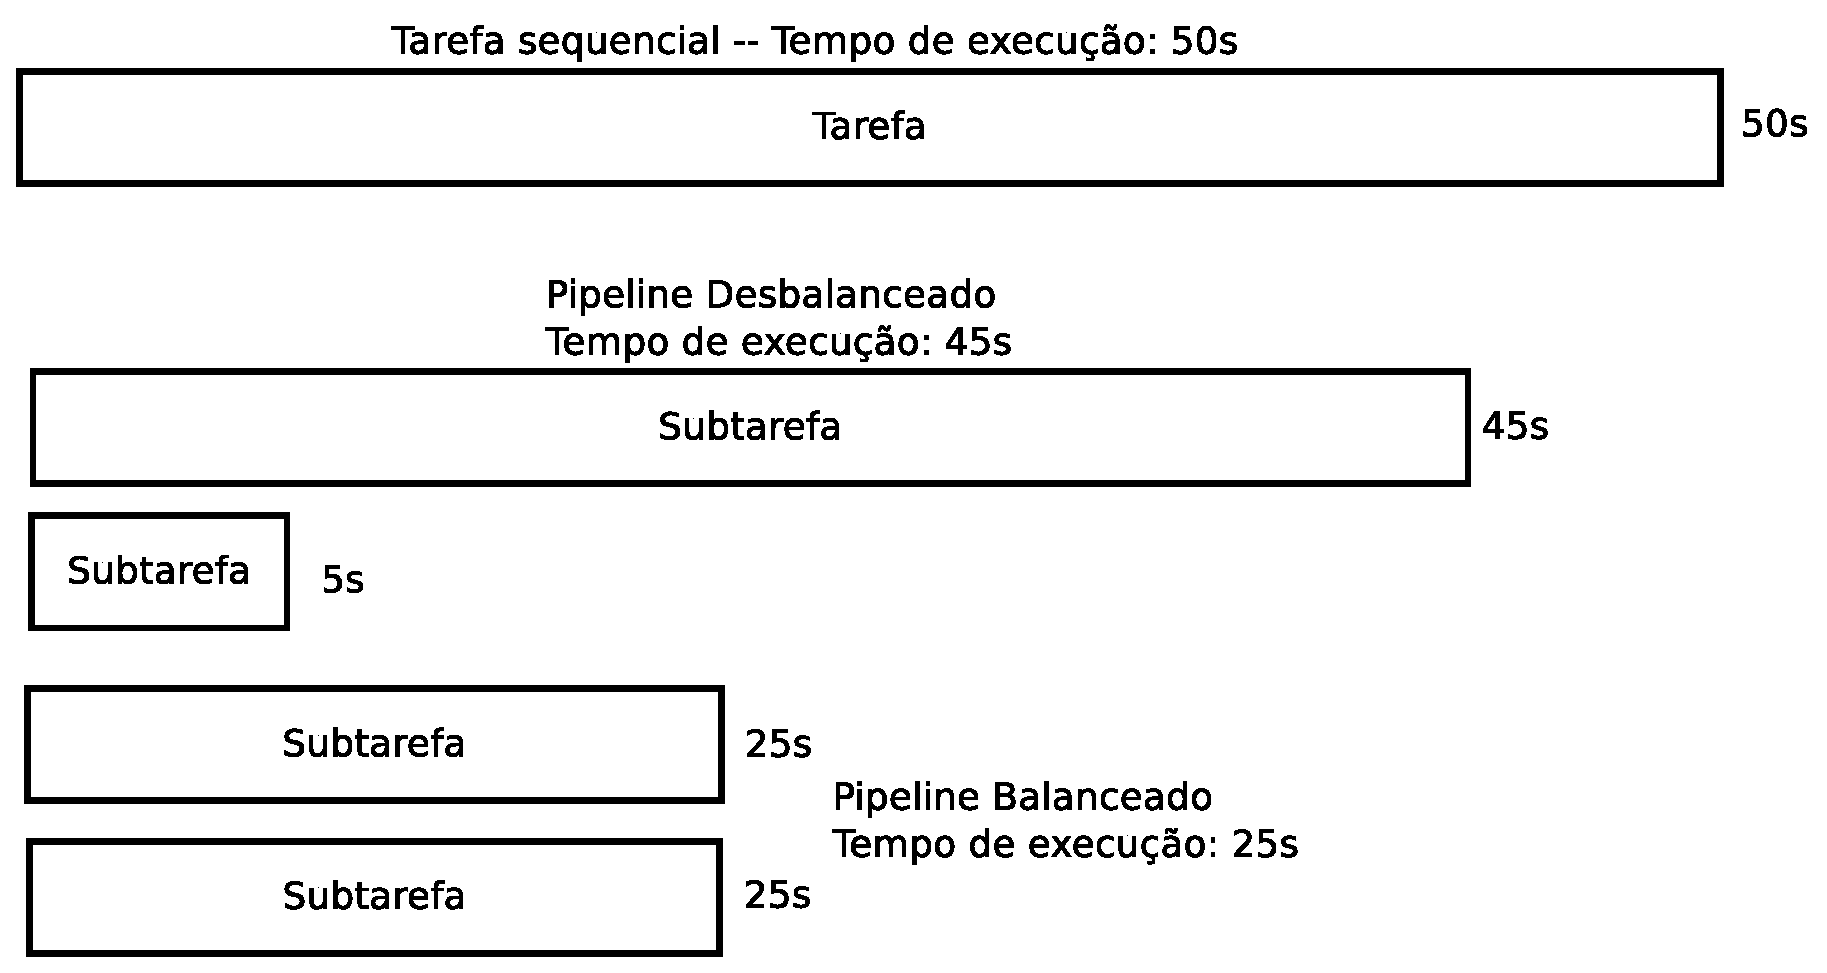
\includegraphics[width=0.95\linewidth]{figs/pipe}
	\caption{Balanceamento de subtarefas.}
	\label{fig:bal}
\end{figure}

O primeiro caso da Figura~\ref{fig:bal} mostra o tempo de execução de uma tarefa
sequencial. Aplicando técnica de pipelining sem levar em conta a questão do
balanceamento, como mostra o segundo caso, o tempo para executar tarefa reduz
pouco se levarmos em conta o tempo da tarefa sequencial. Contudo, se o pipeling
for aplicado com as subtarefas balanceados, o desempenho de execução melhora
consideravelmente, sendo justificável a aplicação dessa técnica para este caso,
visto que o tempo de execução é reduzido pela metade.

\end{section}
\begin{section}{Aplicações de Pipelining}
Esta seção tem como objetivo mostrar a metodogia para implementação do trabalho
proposto.

\begin{subsection}{Forma Sequencial Implementada}


\begin{figure}[!h]
	\centering
	\includegraphics[width=0.95\linewidth]{figs/Sequential.png}
	\caption{Forma sequencial do algoritmo.}
	\label{fig:gray}
\end{figure}



A maioria das imagens digitais é composta por três canais de cores separados: um
canal vermelho, um canal verde e um canal azul. A sobreposição desses canais em
camadas cria uma imagem colorida. Modelos de cores diferentes têm canais
diferentes (às vezes os canais são cores, às vezes são outros valores como
luminosidade ou saturação), mas este trabalho se concentra apenas no RGB.

Todos os algoritmos de conversão do canal RGB para escala de cinza utilizam 
o mesmo processo básico que consistem em três etapas:

\begin{itemize}
\item Obter os valores dos canais vermelho, verde e azul de um \textit{pixel}.
\item Relacionar esses valores para transformar em apenas um valor.
\item Substituir os valores originais de vermelho, verde e azul pelo valor calculado
\end{itemize}


\begin{lstlisting}
for each pixel na imagem{

	vermelho = pixel.Red()
	verde = pixel.Green()
	azul = pizel.Blue()

	Obter_Valor_Cinza = cinza

	pixel.Red = cinza
	pixel.Green = cinza
	pixel.Blue = cinza

}
\end{lstlisting}

Os métodos para obtenção do valor cinza para cada algorimo são apresentados a
seguir.


\begin{figure}[!h]
	\centering
	\includegraphics[width=0.95\linewidth]{figs/gray.png}
	\caption{Resultado dos algoritmos.}
	\label{fig:gray}
\end{figure}

\subsubsection{Algoritmo 1: Média}
O algoritmo baseado na média é a rotina de conversão mais comum em escala de
cinza e o calculo do valor de cinza é obtido a partir da Equação~\ref{eq:media}.

\begin{equation}
\label{eq:media}
cinza = (vermelho + verde + azul)/3
\end{equation}

Essa fórmula gera um equivalente em escala de cinza razoavelmente boa e sua
simplicidade facilita a implementação e otimização. No entanto, esse método não
deixa de ter falhas --- embora rápida e simples, ela faz um mau trabalho em
representar tons de cinza em relação à maneira como os seres humanos percebem a
luminosidade (brilho).


\subsubsection{Algoritmo 2: Luminância}
Esse segundo algoritmo mostra que a densidade do cone no olho humano não é
uniforme entre as cores. Os seres humanos percebem o verde mais fortemente que o
vermelho e o vermelho mais fortemente que o azul. Isso faz sentido do ponto de
vista da biologia evolucionária --- grande parte do mundo natural aparece em
tons de verde, de modo que os humanos desenvolveram maior sensibilidade à luz
verde.

Como os humanos não percebem todas as cores da mesma forma, o ``método da média'' de
conversão em escala de cinza é impreciso. Em vez de tratar as luzes vermelha,
verde e azul igualmente, uma boa conversão em escala de cinza pondera cada cor
com base na maneira como o olho humano a percebe. Uma fórmula comum em
processadores de imagem (Photoshop, GIMP) é apresentada na
Equação~\ref{eq:luminancia}.


\begin{equation}
\label{eq:luminancia}
cinza = (0.3*vermelho + 0.59*verde + 0.11*azul)/3
\end{equation}

\subsubsection{Algoritmo 3: Luma}

Assim como no algoritmo 2, este método tenta uniformizar a forma como o ser
humano perceber as cores. Para isso, também é utilizada uma média ponderada
entre os canais como é mostrado na Equação~\ref{eq:luma}

\begin{equation}
\label{eq:luma}
cinza = (0.2126*vermelho + 0.7152*verde + 0.0722*azul)/3
\end{equation}


\subsubsection{Algoritmo 4: Dessaturação}

A maioria dos programadores usa o modelo de cores RGB. Embora seja uma boa
maneira de uma máquina descrever cores, o espaço de cores RGB pode ser difícil
para a percepção humana. Nesse sentido, o espaço de color HSL (do inglês
\textit{hue, saturation, lightness}) é algumas vezes utilizado para a
vizualização das cores. A matiz (\textit{Hue}) pode ser considerada o nome da
cor --- vermelho, verde, laranja, amarelo etc.  A saturação
(\textit{saturation}) descreve como uma cor é vívida; uma cor muito vívida tem
saturação total, enquanto o cinza não tem saturação. 

A dessaturação de uma imagem funciona convertendo o espaço RGB no espaço HSL e 
forçando a saturação para zero. Um pixel pode ser dessaturado encontrando o
ponto médio entre o máximo de (R, G, B) e o mínimo de (R, G, B), como mostra a
Equação~\ref{eq:dessatura}.

\begin{equation}
\label{eq:dessatura}
cinza = ( Max(vermelho, verde, azul) + Min(vermelho, verde, azul) ) / 2
\end{equation}



\subsubsection{Algoritmo 5: Decomposição}
A decomposição de uma imagem oPde ser considerada uma forma mais simples de
dessaturação. Para decompor uma imagem, cada \textit{pixel} é forçado parao
valor mais alto (máximo) ou mais baixo (mínimo) de seus valores em vermelho,
verde e azul. As Equações~\ref{eq:a} e~\ref{eq:b} mostram como calcular a
decomposição máxima e mínima, respectivamente.

\begin{subequations}

\begin{equation}
\label{eq:a}
cinza = Max(vermelho, verde, azul) 
\end{equation}

\vspace{-1cm}

\begin{equation}
\label{eq:b}
cinza =  Min(vermelho, verde, azul) 
\end{equation}
\end{subequations}


\subsubsection{Algoritmo 6: Canal de cor única}

Este algoritmo representa o método computacional mais simples para conversão em
escala de cinza. Ao contrário de todos os métodos apresentados, este método 
não requer cálculos. Apenas é necessário escolher o valor de um determinado
canal e aplicar para ao valor de cinza, como mostrado na
Equação~\ref{eq:a1},~\ref{eq:b1} e~\ref{eq:c1}

\begin{subequations}

\begin{equation}
\label{eq:a1}
cinza = vermelho 
\end{equation}

\vspace{-1cm}

\begin{equation}
\label{eq:b1}
cinza =  verde 
\end{equation}

\vspace{-1cm}

\begin{equation}
\label{eq:c1}
cinza =  azul 
\end{equation}
\end{subequations}
  
\subsubsection{Algoritmo 7: Tons de cinza}
Este método permite ao usuário especificar quantos tons de cinza a imagem
resultante utilizará. O algoritmo definir o número de tons de cinza da imagem
convertida. Esse método é um pouco mais trabalhoso se comparado com os demais
algoritmos apresentados. Os procedimentos do algoritmo é mostrado a seguir.


\begin{lstlisting}
for each pixel na imagem{
	fator = 255 / (TonsDeCinza - 1)
	metodo = (vermelho + verde + azul)/3
	cinza = (int)((medio / fator) + 0.5) * fator

	//TonsDeCinza: valor entre 2 e 256
}
\end{lstlisting}

\end{subsection}






\end{section}
\begin{section}{Conclusão}
Como descrito, a técnica denominada de pipeline é bastante simples e robusta que
pode ser utilizada em aplicações que demandem melhoria de desempenho na execução
dos processosi. A questão do balanceamneto sempre deve ser levada em
consideração para que o aplicação dessa técnica seja eficaz, contudo nem sempre
é fácil balancear as subtarefas. Portanto, se uma aplicação necessitar ser
executada com um desempenho superior às tarefas seriais, o pipelining pode ser
uma boa alternativa a ser aplicada nesse caso.


\end{section}
\newpage
\bibliographystyle{sbc}
\bibliography{sbc-template}

\end{document}
